\documentclass[../main.tex]{subfiles}

\begin{document}

\subsection{Data Collection}
\subsubsection{Participants}

\subsubsection{Stimulus}
Participants were shown randomly oriented Gabor patches at 7 degrees eccentricity in the right visual field.
%TODO: figure of an example stimulus

\subsubsection{Experimental Design}

\subsubsection{Imaging}

\subsection{MEG Analysis}
\subsubsection{Preprocessing}
MEG analysis was performed in Python with the MNE package. Analysis was performed on 204 planar gradiometers (the 102 magnetometers were not used for analysis). Epochs were rejected for a subject if maximum peaks for any gradiometer exceeded a threshold of $4000\times10^{-13}  \frac{T}{m}$. MEG data was then band-pass filtered from 2-40hz, removing any potential low-frequency artifacts and unused high-frequency data. Independent Component Analysis (ICA) for each subject was calculated to remove artifacts caused by EMG and EOG artifacts. ICA performs source separation for statistically independent components of signals. Eighty Independent components were generated for each subject, and independent components resembling EMG and EOG artifacts were visually selected and then excluded from the filtered MEG dataset. An example of these components is seen in figure \ref{ica_exclude}. Here, we see that the left component represents artifacts resulting from eye blinks, while the right component represents muscle movements from the head that we wish to exclude. Trials were epoched at the onset of the the gabor patch stimulus. Trials were performed in batches of 100 trials that were concatenated for each subject. Analysis was performed on these aggregated sessions.

\begin{figure}
    \centering
    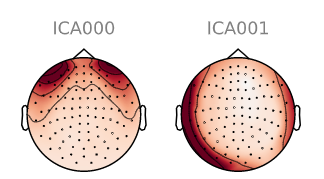
\includegraphics{figures/methods/ica_figure.PNG}
    \caption{Example ICA Components to be Excluded}
    \label{ica_exclude}
\end{figure}

\begin{figure}
    \centering
    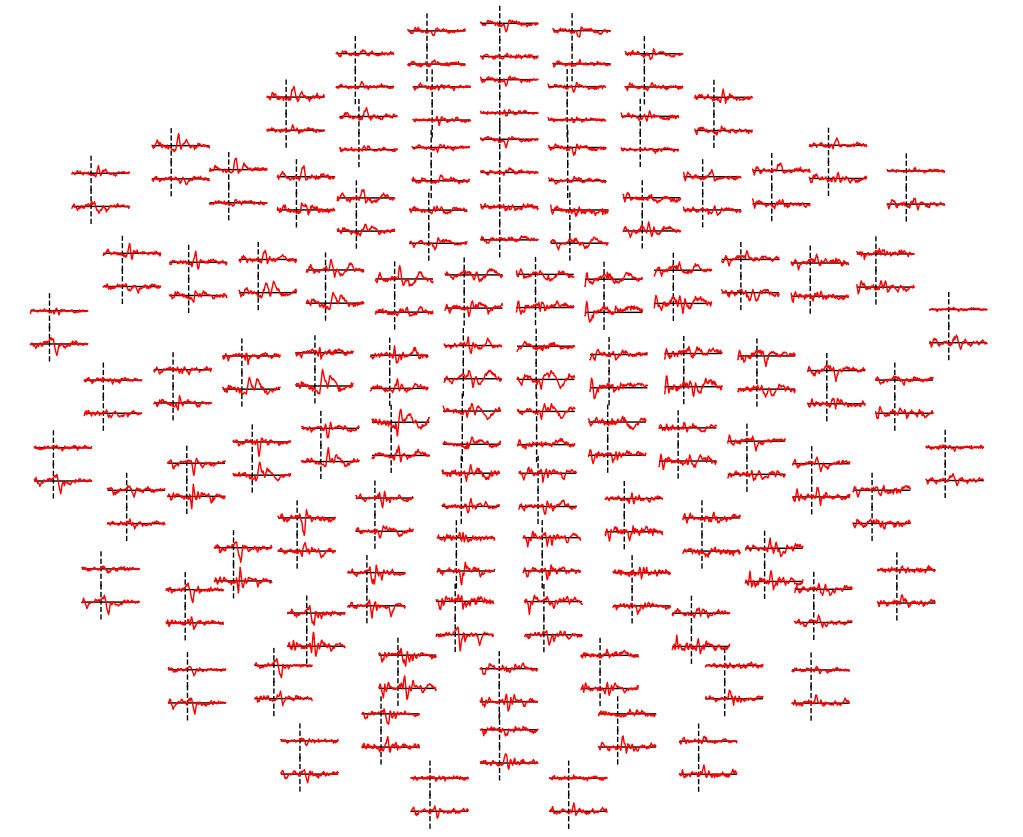
\includegraphics[scale=0.8]{figures/methods/good_topomap.PNG}
    \caption{Example of a Good ERF for a Subject}
    \label{good_topomap}
\end{figure}

\subsubsection{ERF Analysis}
The averaged evoked responses for each subject were measured to ensure that visual responses
appeared in the occipital area as expected. Time-locked epoch responses were averaged over all
trial blocks for each subject at each electrode and visually analyzed for aberrations. In a good subject, like in figure \ref{good_topomap}, we get evoked responses in left hemisphere occipital and temporal electrodes around 0.2 seconds after the stimulus is shown. The stimulus was only shown in the right visual field, so we see limited activation in the right hemisphere.

\subsection{Source Localization Analysis}
\subsubsection{Preprocessing}
%TODO: elaborate more on what recon-all does, citations
Source Localization processing was conducted with freesurfer and mne-python. All subjects were first processed with the freesurfer recon-all command, which performs the freesurfer cortical reconstruction process. After this step, we visually validated every cortical model to check for any artifacts. A BEM head model is then generated for each subject with MNE, using the \texttt{make\_{}watershed\_{}bem} routine. After generating this head model, we have to align our MEG electrodes with the MRI model with a co-registration process. If we didn't line these models up properly, our inverse solution wouldn't be computed correctly, and we might find  activations on an incorrect part of the cortex. After this co-registration process, the MNE BEM routine is run a second time, as the new head coordinates generated by co-registration have to be saved into our BEM model.

\subsubsection{Source Localiztion Pipeline}
%Flesh this out, include a figure?
After this initial pre-processing, we calculate the inverse operator

\subsection{Source Localization Validation}
%mention potential confound that our validation of source localization was based on subjective alignment and assumed knowledge of where we would expect to find visual activations in the cortex


\subsection{Machine Learning Analysis}
\subsubsection{Machine Learning Methods}
%TODO: show a figure of the bowties for binning
Analysis was performed in Python using the Keras library from TensorFlow, decoding libraries from MNE-Python, and the sklearn library. Data was split into training sets of 500 trials for each subject with 100 trials of test trials. Trials were time-binned from 0-0.4 seconds at 0.025 second intervals to account for the 40hz MEG data. The data is split into classes based on a range of orientation angles shaped like "bowties".
% TODO: discuss how we came to the decision of using these classes, as opposed to the original binning or using a regression with sine and cosine values, i.e. because regression didn't give very good results with the small amount of data we had, and we found it better to see the effects of cardinal vs oblique orientations
Because a Gabor patch oriented at $n$ degrees is functionally identical to a gabor patch oriented at $n + 180$ degrees, these bowtie ranges for classification ensure that we do not put two functionally identical Gabor patches into two separate bins. We center these bowties around the horizontal and vertical axis, as well as the two diagonals.For 4 classes, class 0 corresponds to Gabor patches oriented from (337.5-22.5) degrees and (157.5-202.5) degrees, class 1 from (22.5-67.5) and (202.5-247.5) degrees, class 2 from (67.5-112.5) and (247.5-292.5) degrees, class 3 from (112.5-157.5) and (292.5-337.5) degrees. Models were trained for each subject to account for individual Model accuracy was calculated with 5-fold cross-validation and evaluation accuracy on the test dataset. Model accuracy was then compared with the results of a permutation test, in which we shuffled around the training and test labels of the dataset to calculate a baseline accuracy for a naive model. This test essentially compares our models to a chance accuracy.

%TODO: include source localization figure
We used source localization to clarify the readings we received from the electrodes. To validate that the source localization data actually improves our accuracy, or at least gives us equivalent performance, we ran our experiments on inputs from the MEG electrodes (the naive model) and the MRI vertices (the source localization model). There were many more MRI vertices than MEG electrodes, so the weight matrices for the source localization models were much larger than the electrode models. This shouldn't impact the results, but it does mean that we need to tune our hyperparameters differently for electrode and MRI models.
%TODO: explain what hyperparameter tuning is

\subsubsection{Sliding Logistic Regression Model}
The machine learning model used for our control model was a sliding logistic regression model, which calculates a separate accuracy for each timestep of our MEG input signal. For 16 timesteps, we calculate 16 different logistic regression weights, and update these weights using a gradient descent procedure while training. The model was regularized with an elastic net regularization term, which acts as a combination of L1 and L2 regression. This regularization term helps enforce sparsity within our model and prevents weights that are too large, combining the traditional benefits of L1 and L2 regularization. The model also used a "select K best" routine that selects the $K$ best features from the model, based on their contributions to the accuracy. We then had to tune the hyperparameters for these additions to our model, namely the size of $K$, the ratio between L1 and L2 loss for elasticnet, and the regularization parameter $C$. The hyperparameters were tuned to get the best cross-validation accuracy for 500 trials.
%TODO: Final HyperParameters?

%TODO: How does Logistic regression work

The logistic regression model was used for its simplicity and interpretability. The model is relatively easy to implement, especially with the machine learning packages that are already built into scikit-learn and mne-python. The model has only one layer, making it relatively fast to run the model and tune the model parameters. This also means that we can interpret the weights quite easily, as there is a one-to-one correspondence between a particular weight and a reading from an electrode or MRI vertex. This tells us that if a particular weight has a high value, the corresponding electrode/vertex is weighted highly in the model.

%TODO: Remove this? Have not done this analysis yet
\subsubsection{Sliding Neural Network Model}
We also tested our control model with a sliding neural network (SNN). Similar to the sliding logistic regression model, the SNN calculates separate predictions and model weights for each timestep in the input, but we instead train a neural network instead of a logistic regression model. The SNN is much more complex than the logistic regression model, as it has multiple layers, activation functions between each layer, and multiple hyperparameters to tune. Particularly, we have to choose the layer sizes and batch sizes.

%TODO: Brief overview on Neural Networks

\subsubsection{Recurrent Neural Network Model}


\subsection{Serial dependence Analysis}
% TODO: Move to Results
A variety of methods were used to determine how the previous stimulus affected the perception of the current stimulus, i.e. serial dependence. 

\subsubsection{Previous Orientation Decoding}
We first attempted to decode the orientation of the $n-1$th stimulus from the MEG response data corresponding to the $n$th trial. If the previous stimulus orientation biases the current stimulus orientation perception, then it's possible that a decoding model could reverse engineer this bias and decode the orientation of the previous stimulus. This analysis was computed with the same decoding model as the current stimulus decoding, but we shifted the data labels backward by one timestep in relation to the data, such that the data at time $t$ was used to predict the label at time $t - 1$. As a control test, we performed the same analysis with the labels shifted forward by one timestep in relation to the data, so that we tried to predict the next stimulus with the current data, which should give chance performance.

\subsubsection{Bias Analysis}
% Flesh out description and include some figures
We next investigated how the previous stimulus orientation affected the decoding of the current stimulus. This involved

\subsubsection{Sensitivity Analysis}


\subsubsection{Split Half Analysis}
%Split half analysis for close vs. far and for cardinal and oblique analysis


\end{document}